%%% RESULTS %%%

\subsection*{CFRP}

Dipping configuration tests demonstrated the most viable method of CFRP creation to be a 10 times dipped 1K carbon fiber tow in a 16\% ABS solution. This filament had relatively quick coating and drying times, a reasonable diameter equivalent to purchased ABS filament, and a centered carbon fiber tow. Figure~\ref{fig:filament-dipping-dried} is a photo of this CFRP.

\begin{figure}[t]
\centering
\includegraphics[width=0.8\linewidth]{./figures/filament-dipping-dried}
\caption{The finalized CFRP filament.}
\label{fig:filament-dipping-dried}
\end{figure}

Tensile tests were attempted with the finalized CFRP to the near aluminum levels of stiffness shown in early developed fibers (once or twice coated in ABS). However, with significantly more matrix material, ABS simply sheared off at the mounting points so useful data could not be gathered.

\subsection*{Finite Element Analysis}

Figure~\ref{fig:puck-results} shows the composite FEA results. Results indicate the 400 N is the maximum load that can be applied to the specimen prior to failure. Figure~\ref{fig:fea-acp-pfailure-notext} shows the central arch closest to failure, as expected. Figure~\ref{fig:fea-acp-pfailure-mode-layer-closeup} shows which Puck inter-fiber failure (IFF) in which layer of the printed part is applicable to each element (pmC denotes matrix shear failure, and pd denotes delamination).

\begin{figure}[t]
        \centering
        \begin{subfigure}[b]{0.4\linewidth}
                \includegraphics[width=\linewidth]{./figures/fea/fea-acp-pfailure-notext}
                \caption{Contour plot.}
                \label{fig:fea-acp-pfailure-notext}
        \end{subfigure}
        \begin{subfigure}[b]{0.4\linewidth}
                \includegraphics[width=\linewidth]{./figures/fea/fea-acp-pfailure-mode-layer-closeup}
                \caption{Close up.}
                \label{fig:fea-acp-pfailure-mode-layer-closeup}
        \end{subfigure}
        \caption{Puck failure results from FEA.}\label{fig:puck-results}
\end{figure}

Figure~\ref{fig:puck-failure-qualitative} graphically represents which areas and layers of the part are prone to failure based on FEA results (delamination in blue and matrix shear in orange). The orange block shows the forces acting on a sample element in bending tension (matrix shear), and blue represents a middle layer being pulled apart from adjacent tensions (delamination). These two Puck IFF cases, $\theta_{fp}=90^{\circ}$ positive transverse shear and $\theta_{fp}=90^{\circ}$ through thickness tensions, significantly impact the load bearing capacity of UD CFRP parts, therefore validating the FEA prediction of the printed specimen's mechanical behavior \cite{Puck-Stuttgard}. FEA using ABS and aluminum were also implemented. A comparison of the results suggest that the curved layer CFRP 3D printed specimen will be nearly twice as strong as an ABS part with stiffness on the order of an aluminum part.

\begin{figure}[t]
\centering
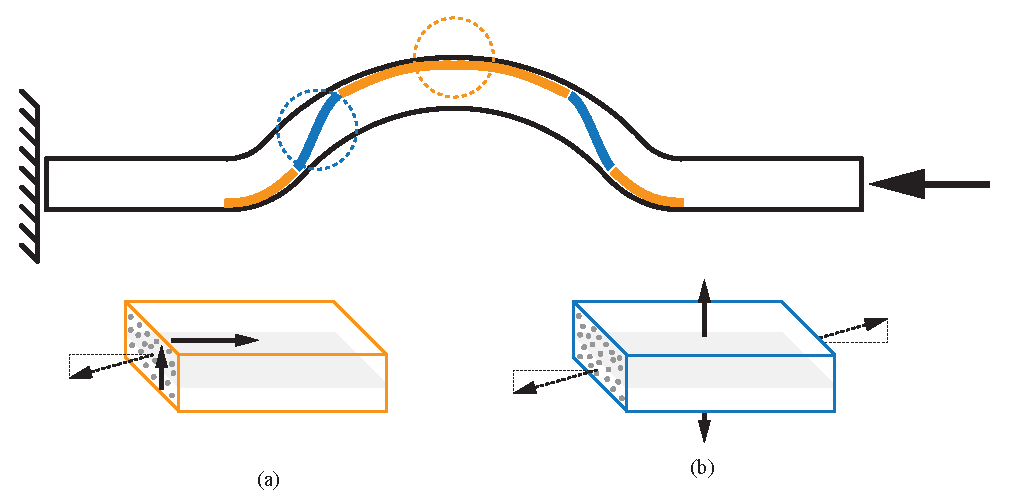
\includegraphics[width=0.8\linewidth]{./figures/fea/puck-failure-qualitative}
\caption{Diagrams of Puck IFF in the bridge specimen.}
\label{fig:puck-failure-qualitative}
\end{figure}


\subsection*{Print Testing}

The finalized CFRP filament was printed tested using the 3Doodler. Figure~\ref{fig:filament-print-3doodler-during} is a photo of this test. To successfully print, ABS must be stripped of the front of the filament and the exposed tow inserted through a room temperature nozzle. The exposed tow was then tacked down with ABS slurry and printing begun. This forward tension was necessary to keep the tow centered in the molten ABS inside the heating chamber. Once printing, the set extruded filament maintained the tension.

\begin{figure}[t]
\centering
\includegraphics[width=0.5\linewidth]{./figures/filament-print-3doodler-during}
\caption{Test printing the CFRP filament with a 3Doodler.}
\label{fig:filament-print-3doodler-during}
\end{figure}

A tensile test on the printed CFRP filament yielded a tensile strength of 338 MPa, Stiffness of 7.63 GPa, and a failure strain of 4.44\%, all comparable to CFRP properties prior to printing. However, limited amounts of ABS were extruded compared to the amount on the CFRP filament prior to printing. Only a full curved layer printing test will tell whether or not this amount of matrix material is suffcient. 